\documentclass{article}

%% Page Margins %%
\usepackage{geometry}
\geometry{
    top = 0.75in,
    bottom = 0.75in,
    right = 0.75in,
    left = 0.75in,
}

\usepackage{amsmath}
\usepackage{graphicx}
\usepackage{parskip}

\title{Assembly Project: Dr Mario}

% TODO: Enter your name
\author{Hiu Yan Kwok and Minseok Kwag}

\begin{document}
\maketitle

\section{Instruction and Summary}

\begin{enumerate}

    \item Which milestones were implemented? \\
    As of Nov. 24, the milestones 1, 2, and 3 were implemented.

    \item How to view the game:
    % TODO: specify the pixes/unit, width and height of 
    %       your game, etc.  NOTE: list these details in
    %       the header of your breakout.asm file too!
    
    Set the display width and height to 64. We have 14 rows and 7 columns in our version.
    
    \begin{enumerate}

    \item
    \item
    \item


    \end{enumerate}

    

\begin{figure}[ht!]
    \centering
    % \includegraphics[width=0.3\textwidth]{name.png}
    \caption{caption}
    \label{Instructions}
\end{figure}

\item Game Summary:
% TODO: Tell us a little about your game.
\begin{itemize}
\item
\item
\end{itemize}

    
\end{enumerate}

Question 2. Store the board as 14 rows of 7 four-byte words, one row after another, for 392 bytes total. Zero means empty. Values 1 through 4 mean pink, green, blue, and yellow. Store the player column, held colour and count, and keystroke count separately.

Question 3.

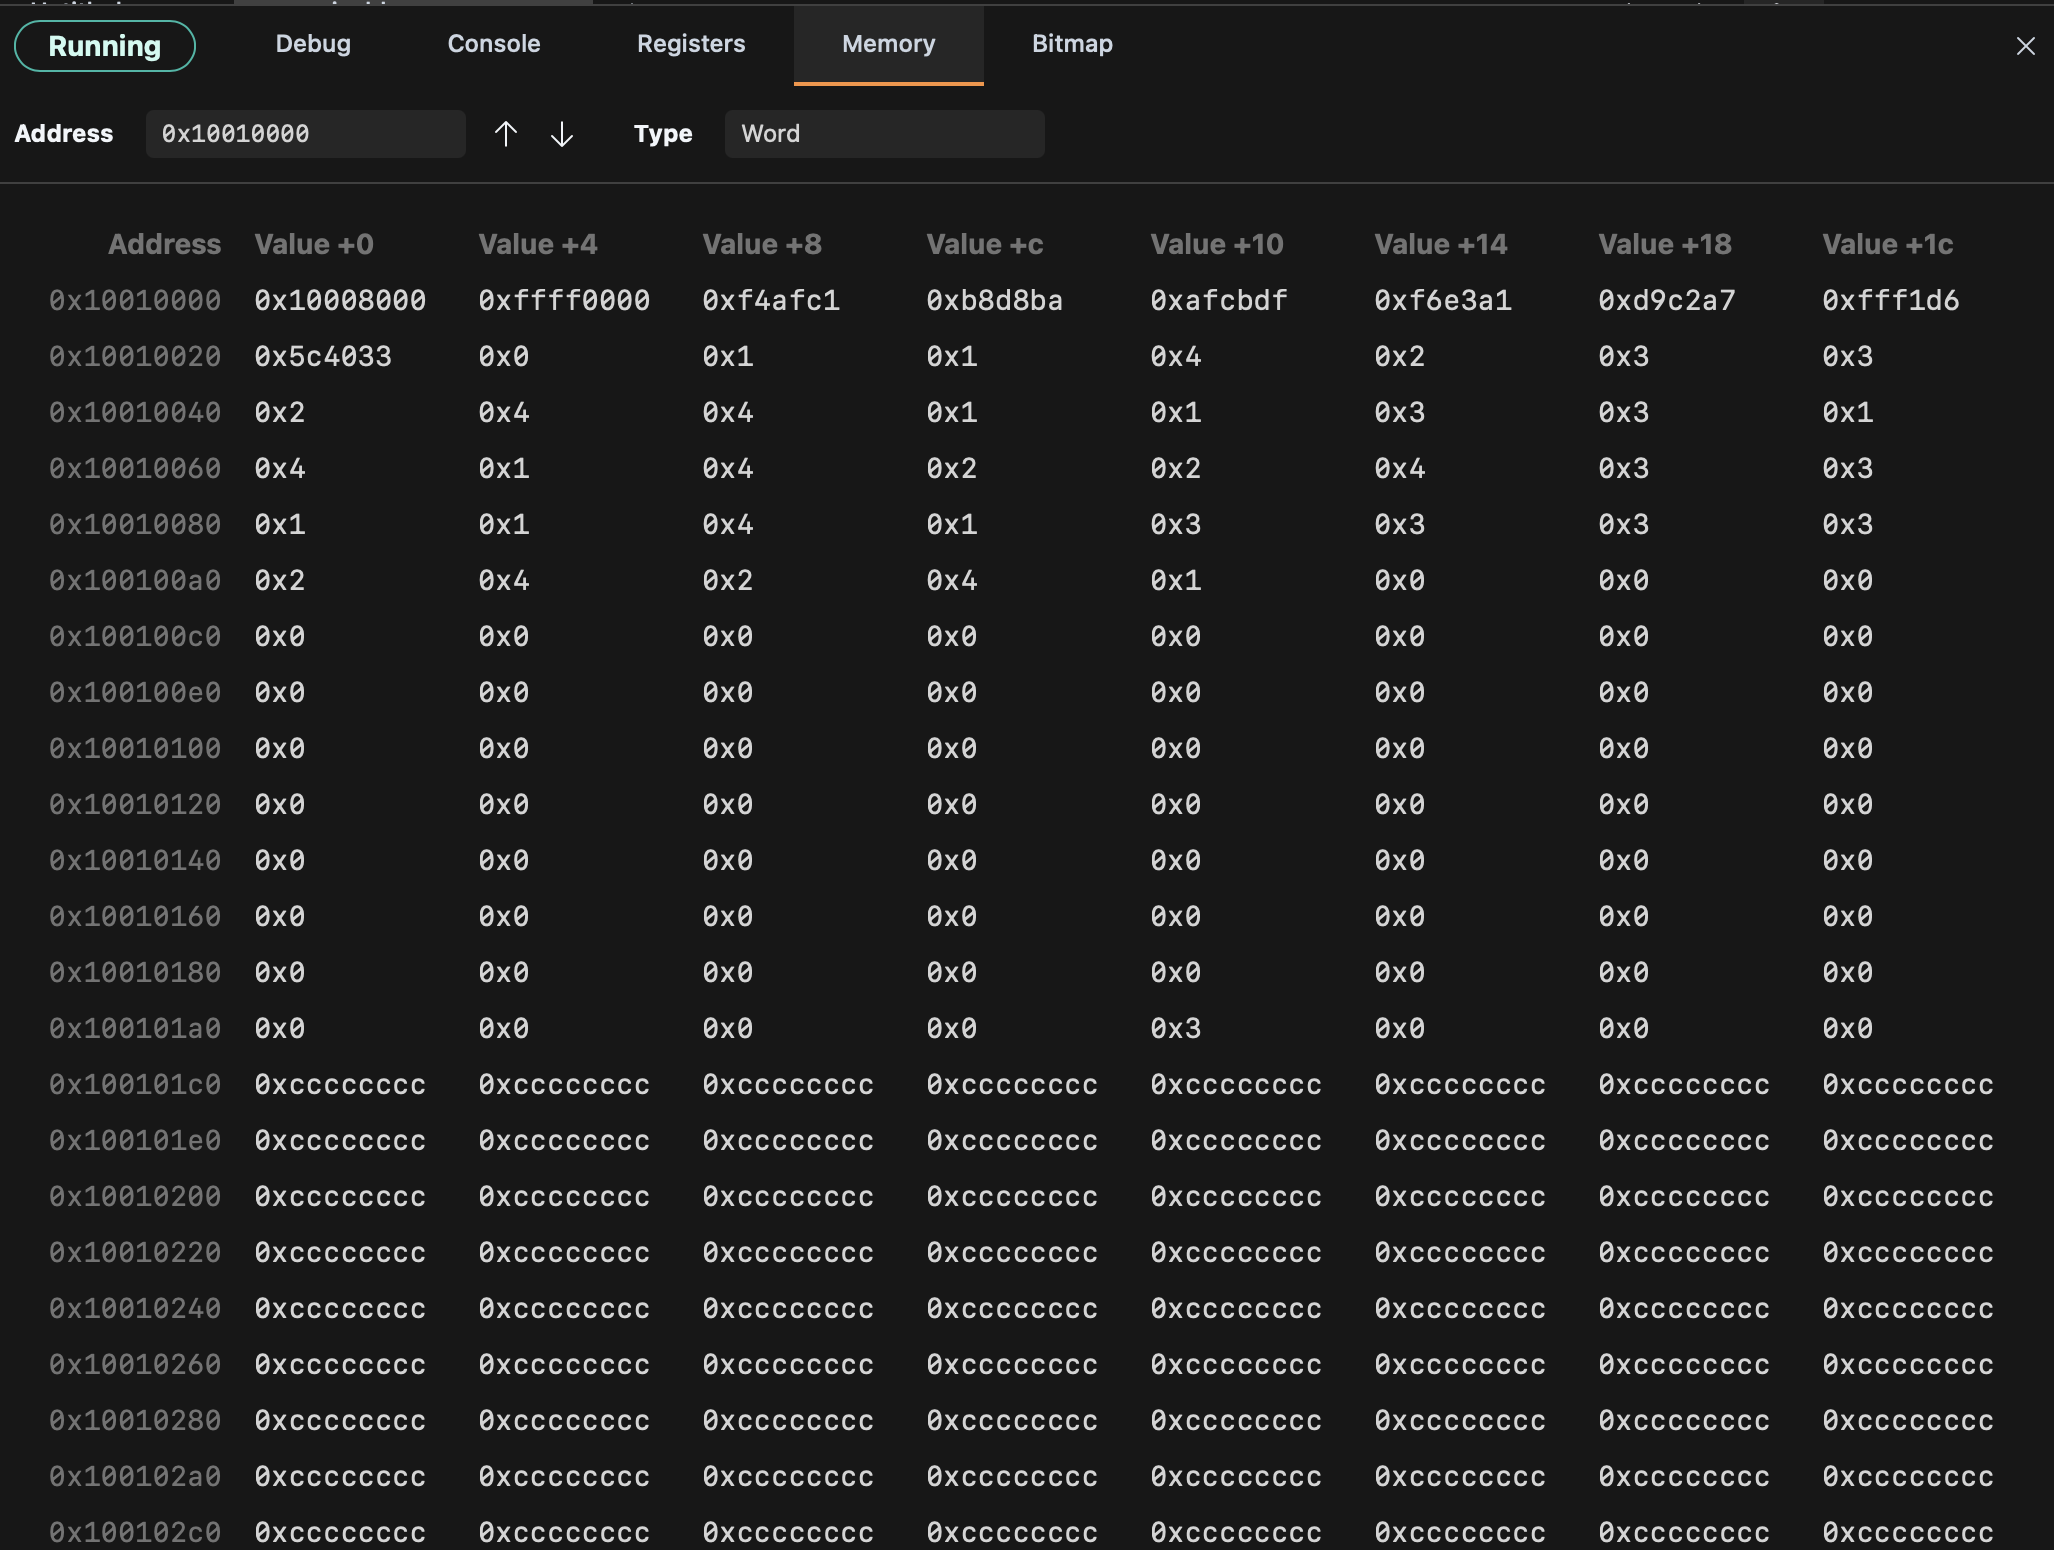
\includegraphics[width=0.8\linewidth]{memory-layout.png}

Question 4. Draw five rows of random coloured squares at the top of the board and a cream player square below the centre column.


\includegraphics[width=0.6\linewidth]{milestone-1-scene.png}

Question 5. A and D move the player left and right. S grabs the lowest bubble in the current column and any matching bubbles directly above it. Every ten counted inputs shift the board down and add a new top row. Q quits.

\section{Attribution Table}
% TODO: If you worked in partners, tell us who was
% responsible for which features. Some reweighting
% might be possible in cases where one group member
% deserves extra credit for the work they put in.
\begin{center}
\begin{tabular}{|| c | c ||}
\hline
Student 1 (Hiu Yan Kwok 1010969855) & Student 2 (Minseok Kwag 1009608444) \\
\hline
Gameplay design & \\
\hline
Milestone 1: Board and player initialization & Milestone 3\\
\hline
Milestone 2: Movement, grabbing, and row advancement & Hard Features 3 and 4\\
\hline
Task & Task\\
\hline
Task & Task\\
\hline
\end{tabular}
\end{center}
% TODO: Fill out the remainder of the document as you see
% fit, including as much detail as you think
% necessary to better understand your code.
% You can add extra sections and subsections to
% help us understand why you deserve marks for
% features that were more challenging than they
% might initially seem.


\end{document}
